\documentclass[12pt]{article}\usepackage[]{graphicx}\usepackage[]{color}
%% maxwidth is the original width if it is less than linewidth
%% otherwise use linewidth (to make sure the graphics do not exceed the margin)
\makeatletter
\def\maxwidth{ %
  \ifdim\Gin@nat@width>\linewidth
    \linewidth
  \else
    \Gin@nat@width
  \fi
}
\makeatother

\definecolor{fgcolor}{rgb}{0.345, 0.345, 0.345}
\newcommand{\hlnum}[1]{\textcolor[rgb]{0.686,0.059,0.569}{#1}}%
\newcommand{\hlstr}[1]{\textcolor[rgb]{0.192,0.494,0.8}{#1}}%
\newcommand{\hlcom}[1]{\textcolor[rgb]{0.678,0.584,0.686}{\textit{#1}}}%
\newcommand{\hlopt}[1]{\textcolor[rgb]{0,0,0}{#1}}%
\newcommand{\hlstd}[1]{\textcolor[rgb]{0.345,0.345,0.345}{#1}}%
\newcommand{\hlkwa}[1]{\textcolor[rgb]{0.161,0.373,0.58}{\textbf{#1}}}%
\newcommand{\hlkwb}[1]{\textcolor[rgb]{0.69,0.353,0.396}{#1}}%
\newcommand{\hlkwc}[1]{\textcolor[rgb]{0.333,0.667,0.333}{#1}}%
\newcommand{\hlkwd}[1]{\textcolor[rgb]{0.737,0.353,0.396}{\textbf{#1}}}%
\let\hlipl\hlkwb

\usepackage{framed}
\makeatletter
\newenvironment{kframe}{%
 \def\at@end@of@kframe{}%
 \ifinner\ifhmode%
  \def\at@end@of@kframe{\end{minipage}}%
  \begin{minipage}{\columnwidth}%
 \fi\fi%
 \def\FrameCommand##1{\hskip\@totalleftmargin \hskip-\fboxsep
 \colorbox{shadecolor}{##1}\hskip-\fboxsep
     % There is no \\@totalrightmargin, so:
     \hskip-\linewidth \hskip-\@totalleftmargin \hskip\columnwidth}%
 \MakeFramed {\advance\hsize-\width
   \@totalleftmargin\z@ \linewidth\hsize
   \@setminipage}}%
 {\par\unskip\endMakeFramed%
 \at@end@of@kframe}
\makeatother

\definecolor{shadecolor}{rgb}{.97, .97, .97}
\definecolor{messagecolor}{rgb}{0, 0, 0}
\definecolor{warningcolor}{rgb}{1, 0, 1}
\definecolor{errorcolor}{rgb}{1, 0, 0}
\newenvironment{knitrout}{}{} % an empty environment to be redefined in TeX

\usepackage{alltt}

\usepackage{geometry}                % See geometry.pdf to learn the layout options. There are lots.
\geometry{a4paper,
 total={170mm,257mm},
 left=20mm,
 right=20mm,
 top=20mm,
 bottom=40mm}                   % ... or a4paper or a5paper or ...
\geometry{landscape}                % Activate for for rotated page geometry
\usepackage[parfill]{parskip}    % Activate to begin paragraphs with an empty line rather than an indent
\usepackage{graphicx}
\usepackage{amssymb}
\usepackage{epstopdf}
\usepackage{float}
\usepackage{hyperref}
\usepackage{booktabs}
\usepackage{colortbl, xcolor}
\usepackage{array}
\usepackage{lastpage}


\setlength{\columnsep}{1cm}
\usepackage[backend=bibtex, sorting=none, style=chicago-authordate]{biblatex}
\setlength\bibitemsep{\baselineskip}
\usepackage[british]{babel}
\usepackage[export]{adjustbox}
\usepackage{listings}
\usepackage{color}
\definecolor{codegreen}{rgb}{0,0.6,0}
\definecolor{codegray}{rgb}{0.5,0.5,0.5}
\definecolor{codepurple}{rgb}{0.58,0,0.82}
\definecolor{backcolour}{rgb}{0.95,0.95,0.92}
\lstdefinestyle{mystyle}{
    backgroundcolor=\color{backcolour},
    commentstyle=\color{codegreen},
    keywordstyle=\color{magenta},
    numberstyle=\tiny\color{codegray},
    stringstyle=\color{codepurple},
    basicstyle=\footnotesize,
    breakatwhitespace=false,
    breaklines=true,
    captionpos=b,
    keepspaces=true,
    numbers=left,
    numbersep=5pt,
    showspaces=false,
    showstringspaces=false,
    showtabs=false,
    tabsize=2
}


\newcolumntype{L}[1]{>{\raggedright\let\newline\\
    \arraybackslash\hspace{0pt}}m{#1}}
\newcolumntype{C}[1]{>{\centering\let\newline\\
    \arraybackslash\hspace{0pt}}m{#1}}
\newcolumntype{R}[1]{>{\raggedleft\let\newline\\
    \arraybackslash\hspace{0pt}}m{#1}}
\newcolumntype{P}[1]{>{\raggedright\tabularxbackslash}p{#1}}

%\usepackage{pdflscape}
 \usepackage{rotating}
  
\usepackage{textcomp}
\lstset{style=mystyle}


\hypersetup{%
  colorlinks=true,% hyperlinks will be coloured
  linkcolor=blue,% hyperlink text will be green
}
\DeclareGraphicsRule{.tif}{png}{.png}{`convert #1 `dirname #1`/`basename #1 .tif`.png}

%% LOGOS
\usepackage{fancyhdr}
%\setlength{\headheight}{1.5cm}
\addtolength{\headheight}{2cm} % make more space for the header
\pagestyle{fancyplain} % use fancy for all pages except chapter start
\lhead{
\includegraphics[height=1.3cm, width=2cm]{../logos/NBIS-logo.png}} % left logo
\rhead{
\includegraphics[height=1.3cm, width=4cm]{../logos/SciLifeLab-logo.jpg}} % right logo
\cfoot{\thepage\ (\pageref{LastPage})}
%\lfoot{Biostatistics Essentials: a blackboard approach}
\renewcommand{\headrulewidth}{0pt} % remove rule below header


%% BEGIN DOCUMENT
\IfFileExists{upquote.sty}{\usepackage{upquote}}{}
\begin{document}




%% SUPPORT REQUEST
%\newpage


Exercise: simple linear regression:  body weight and plasma volume. 
Example data contain the body weight (kg) and plasma volume (literes) for eight healthy men. 

\section{Estimating model coefficients}
% latex table generated in R 3.5.1 by xtable 1.8-3 package
% Thu May 16 14:19:09 2019
\begin{table}[ht]
\centering
\begingroup\large
\begin{tabular}{|C{2.5cm}|C{2.5cm}|C{2.5cm}|C{2.5cm}|C{3cm}|C{2.5cm}|C{2.5cm}|C{2.5cm}}
  \toprule
weight [kg] & plasma [l] & $x_i-\overline{x}$ & $y_i-\overline{y}$ & $(x_i-\overline{x})(y_i-\overline{y})$ & $(x_i-\overline{x})^2$ & $(y_i-\overline{y})^2$ & $x^2$ \\ 
  \midrule
58.00 & 2.75 &  &  &  &  &  &  \\ 
   \rowcolor[gray]{0.95}70.00 & 2.86 &  &  &  &  &  &  \\ 
  74.00 & 3.37 &  &  &  &  &  &  \\ 
   \rowcolor[gray]{0.95}63.50 & 2.76 &  &  &  &  &  &  \\ 
  62.00 & 2.62 &  &  &  &  &  &  \\ 
   \rowcolor[gray]{0.95}70.50 & 3.49 &  &  &  &  &  &  \\ 
  71.00 & 3.05 &  &  &  &  &  &  \\ 
   \rowcolor[gray]{0.95}66.00 & 3.12 &  &  &  &  &  &  \\ 
   \bottomrule
\end{tabular}
\endgroup
\end{table}


1. Calculate: 

$\overline{y}=\frac{1}{n}\sum_{i=1}^{n}y_i = $ \newline
\vspace{0.2cm} 

$\overline{x}=\frac{1}{n}\sum_{i=1}^{n}x_i = $ \newline
%\vspace{0.5cm}

2. Fill in columns 3rd to 6th (leave the last 2 columns for now)

3. Calculate $\hat{\beta_1}$: \newline
\vspace{0.1cm} 

$\hat{\beta_1}= \frac{\sum_{i=1}^{n}(x_i-\overline{x})(y_i-\overline{y})}{\sum_{i=1}^{n}(x_i-\overline{x})^2}=$ \newline
\vspace{0.5cm}

4. Calculate $\hat{\beta_0}$: \newline
\vspace{0.1cm} 
$\hat{\beta_0}=\overline{y}-\hat{\beta_1}\overline{x}=$ \newline

5. Write equation for the best-fitting straight line:



\section{Accuracy of the coefficient estimates}

1. Fill in the remainig columns in the table above
\vspace{1cm} 

2. Calculate $s$ \newline

$s=\sqrt{[\frac{\sum_{i=1}^{n}(y_i-\overline{y})^2-\overline{\beta_1}\sum_{i=1}^{n}(x_i-\overline{x})^2}{n-2}]}=$
\vspace{1cm} 

3. Calculate 
$s.e(\hat{\beta_0})=s*\sqrt{[\frac{1}{n}+\frac{x_i^2}{\sum_{i=1}^{n}(x_i-\overline{x})^2}]}=$
\vspace{1cm} 

4. Calculate
$s.e(\hat{\beta_1})=\frac{s}{\sqrt{\sum_{i=1}^{n}(x_i-\overline{x})^2}}=$
\vspace{0.2cm} 

5. Have a look at Figure 3.3 in \textit{An Introduction to Statistical Learning} and answer questions
\begin{itemize}
  \item What do 10 light blue lines represent on the plot (right)?
  \item What is an \texttt{unbiased estimator}?
  \item Have we underestimated or overestimated ${\beta_1}$?
\end{itemize}

\section{Hypothesis testing}
Is there an association between body weight and plasma volume? 

1. Write down the null hypothesis and alternative hypothesis

2. Calculate t-statistics for $\hat{\beta_1}$ \newline

$t=\frac{\hat{\beta_1}-0}{s.e.(\hat{\beta_1})} = $
\vspace{0.2cm}

3. Use t distribution table containing critical values of the t distribution, to check if whether the p-value for our calculated t-statistics is lower than 5\% threshold? Is it lower than 1\% threshold?

4. Can we reject the null hypothesis? Is there an association between body weight and plasma volume. 

\newpage
\section{Prediction}

\begin{knitrout}
\definecolor{shadecolor}{rgb}{0.969, 0.969, 0.969}\color{fgcolor}\begin{figure}[H]

{\centering 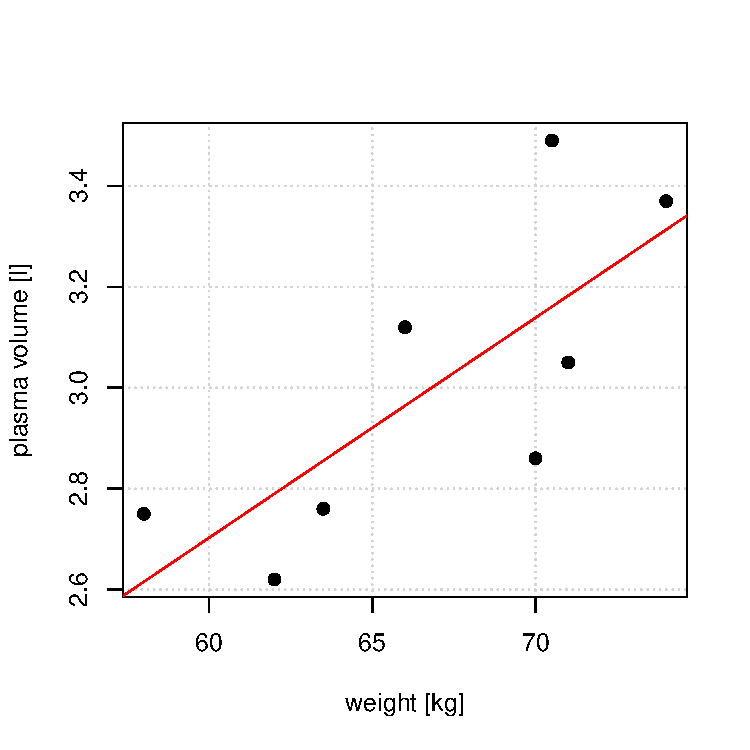
\includegraphics[width=\maxwidth]{figure/fig-prediction-1} 

}

\caption[Body weight vs]{Body weight vs. plasma volume}\label{fig:fig-prediction}
\end{figure}


\end{knitrout}

1. Given Figure \ref{fig:fig-prediction} predict `plasma volume` for weight values of 60, 65, and 70 kg

2. Calculate predicted values of `plasma volume` for weight values of 60, 65 and 70 kg using the equation  $y_i'=\hat{\beta_0}+\hat{\beta_1}x_i'$

$y_{60}'=$ \vspace{0.2cm}

$y_{65}'=$ \vspace{0.2cm}

$y_{70}'=$ \vspace{0.2cm}


3. Calculate standard error for the predicted `plasma volume` for weight value of 60 kg \newline \vspace{0.4cm}

$s.e.(y_i')=s\sqrt{[1+\frac{1}{n}+\frac{(x_i´-\overline{x_i})^2}{\sum_{i=1}^{n}(x_i-\overline{x_i})^2}]}=$ \vspace{0.2cm}

\newpage
\section{Asesssing the Accuracy of the Model \& Correlation}
1. Using Given Figure \ref{fig:fig-prediction} try to calculate (estimate) the RSE. We will check which group gets results closeset to the computed ones. 

2. Using lecture and this pen-and-paper docs, calculate $R^2$, i.e. do not use computer to calculated. Hint: most of the values have been reported / calculated before. It is ok to use mobiles for adding and dividing things up. \newline \vspace{0.2cm}

$R^2=\frac{TSS-RSS}{TSS}=1-\frac{RSS}{TSS}=$ \vspace{0.2cm}

3. Calculate correlation \newline \vspace{0.2cm}

$Cor(X,Y)=\frac{\sum_{i=1}^{n}(x_i-\overline{x})(y_i-\overline{y})}{\sqrt{\sum_{i=1}^{n}(x_i-\overline{x})^2}\sqrt{\sum_{i=1}^{n}(y_i-\overline{y})^2}}=s$

\newpage
\section{Extra dataset to practise more}



% latex table generated in R 3.5.1 by xtable 1.8-3 package
% Thu May 16 14:19:09 2019
\begin{table}[ht]
\centering
\begingroup\large
\begin{tabular}{|C{2.5cm}|C{2.5cm}|C{2.5cm}|C{2.5cm}|C{3cm}|C{2.5cm}|C{2.5cm}|C{2.5cm}}
  \toprule
weight [kg] & height [cm] & $x_i-\overline{x}$ & $y_i-\overline{y}$ & $(x_i-\overline{x})(y_i-\overline{y})$ & $(x_i-\overline{x})^2$ & $(y_i-\overline{y})^2$ & $x^2$ \\ 
  \midrule
110.00 & 182.00 &  &  &  &  &  &  \\ 
   \rowcolor[gray]{0.95}74.00 & 170.00 &  &  &  &  &  &  \\ 
  96.00 & 185.00 &  &  &  &  &  &  \\ 
   \rowcolor[gray]{0.95}100.00 & 178.00 &  &  &  &  &  &  \\ 
  94.00 & 172.00 &  &  &  &  &  &  \\ 
   \rowcolor[gray]{0.95}69.00 & 168.00 &  &  &  &  &  &  \\ 
  83.00 & 170.00 &  &  &  &  &  &  \\ 
   \rowcolor[gray]{0.95}76.00 & 170.00 &  &  &  &  &  &  \\ 
  80.00 & 168.00 &  &  &  &  &  &  \\ 
   \rowcolor[gray]{0.95}71.00 & 158.00 &  &  &  &  &  &  \\ 
   \bottomrule
\end{tabular}
\endgroup
\end{table}



\begin{knitrout}
\definecolor{shadecolor}{rgb}{0.969, 0.969, 0.969}\color{fgcolor}

{\centering 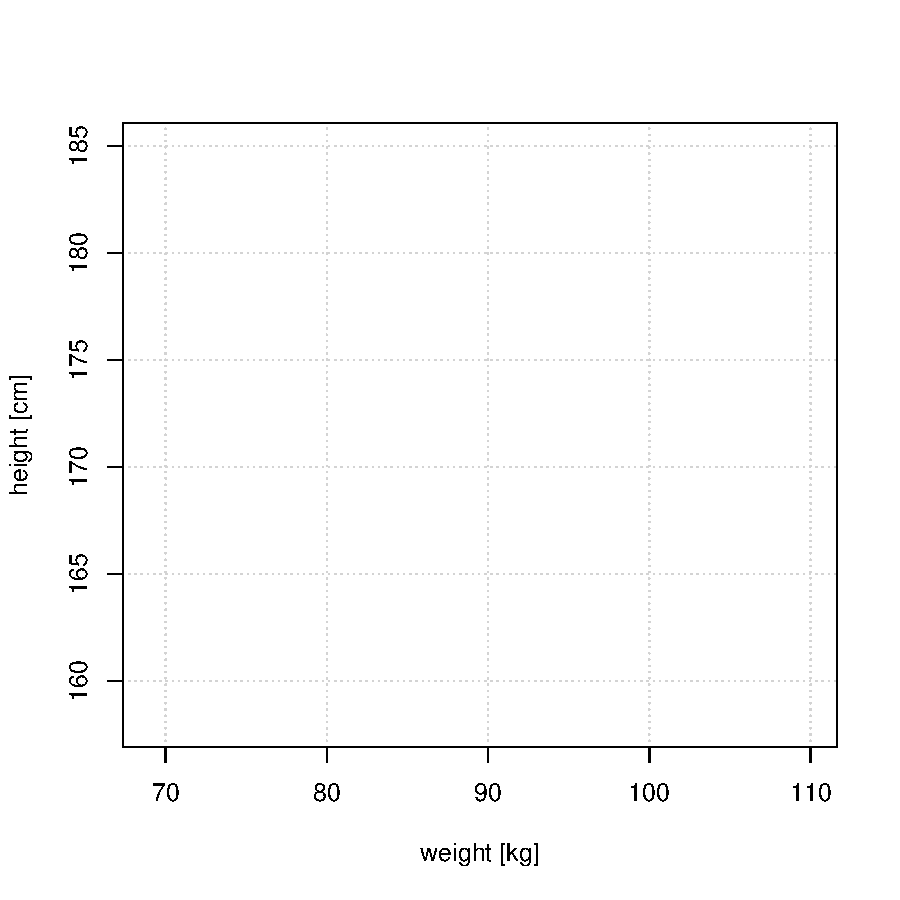
\includegraphics[width=\maxwidth]{figure/exmpty-plot-1} 

}



\end{knitrout}


\end{document}  




